% Author: Izaak Neutelings (June 2017)
% Updated: December 2022
\documentclass[border=3pt,tikz]{standalone}
\tikzset{>=latex} % for LaTeX arrow head

\begin{document}

% PSEUDORAPIDITY with manual for-loop over theta, eta
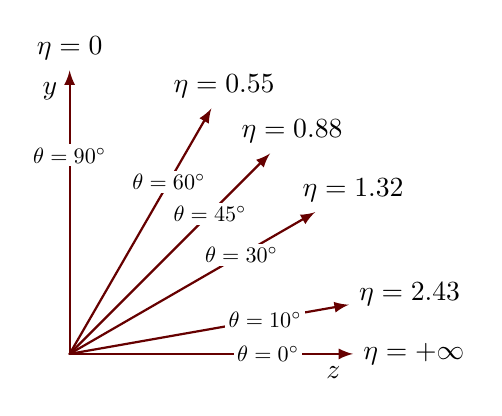
\begin{tikzpicture}[scale=3]
  \def\R{1.2} % radius/length of lines
  \node[scale=1,below left=1] at (0,\R) {$y$}; % y axis
  \node[scale=1,below left=1] at (\R,0) {$z$}; % z axis
  \foreach \t/\e in {90/0,60/0.55,45/0.88,30/1.32,10/2.43,0/+\infty}{ % loop over theta/eta
    \pgfkeys{/pgf/number format/precision=2}
    \draw[->,black!60!red,thick,line cap=round] % eta lines
      (0,0) -- (\t:\R) node[anchor=180+\t,black] {$\eta=\e$}
      node[black,pos=0.7,fill=white,scale=0.8,inner sep=1.5pt] {$\theta=\t^\circ$};
  }
  %\draw[black!60!red,thick] (0,0.1*\R) |- (0.1*\R,0) ; % overlap in corner
\end{tikzpicture}

% PSEUDORAPIDITY with automatic calculation of eta
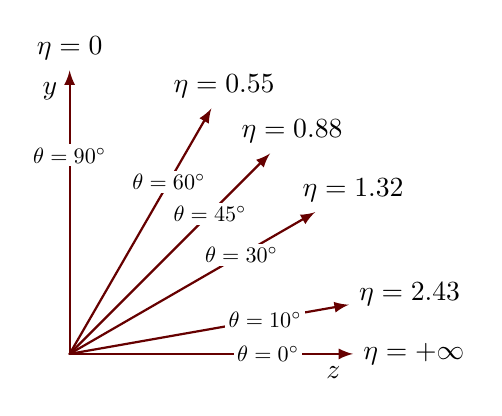
\begin{tikzpicture}[scale=3]
  \pgfkeys{/pgf/number format/precision=2} % two decimals
  \def\R{1.2} % radius/length of lines
  \node[scale=1,below left=1] at (0,\R) {$y$}; % y axis
  \node[scale=1,below left=1] at (\R,0) {$z$}; % z axis
  \foreach \t in {90,60,45,30,10,0}{ % loop over theta
    \ifnum \t = 0
      \def\e{+\infty} % infinity symbol
    \else
      \pgfmathparse{-ln(tan(\t/2))} % pseudorapidity
      %\pgfmathroundto{\pgfmathresult} % round without traling zeroes
      \pgfmathroundtozerofill{\pgfmathresult} % round with trailing zeroes
      \pgfmathsetmacro\e{\t==90?0:\pgfmathresult} % no trailing zeroes for theta = 0
    \fi
    \draw[->,black!60!red,thick,line cap=round] % eta lines
      (0,0) -- (\t:\R) node[anchor=180+\t,black] {$\eta=\e$}
      node[black,pos=0.7,fill=white,scale=0.8,inner sep=1.5pt] {$\theta=\t^\circ$};
  }
  %\draw[black!60!red,thick] (0,0.1*\R) |- (0.1*\R,0) ; % overlap in corner
\end{tikzpicture}

\end{document}
